% !TEX root = ../main.tex
% NB: Denne filen bruker TikZ for to grafiske modeller (agent og prinsipal).
% Orchestrator: vennligst legg til \usepackage{tikz} i notes/preamble.tex.
\section{Optimal effort-modell (agent- og prinsipalside)}\label{thr:optimal-effort-model}

\paragraph{Definisjon.} Optimal effort-modellen er den standardiserte principal-agent-rammen fra BSZ kap.\ 15 som anviser hvordan agentens innsatsnivå $e$ og prinsipalens insentivkoeffisient $\beta$ velges optimalt under risiko og asymmetrisk informasjon. Modellen kombinerer en lineær outputfunksjon $Q=\alpha e+\mu$, en lineær kontrakt $W=W_0+\beta Q$ og en risikoavers agent, og leverer to førsteordensbetingelser -- én for agenten (effort-valg) og én for prinsipalen (kontraktsdesign). [SLIDE]

\subsection*{Forklaring}

Modellen har to aktører som tar beslutninger i sekvens. \emph{Prinsipalen} (eier/virksomhet) velger først kontraktsparametrene $(W_0,\beta)$ og kunngjør dem. \emph{Agenten} (medarbeider) velger deretter innsats $e$ for å maksimere egen forventet nytte, idet $\mu$ realiseres og lønnen $W$ utbetales. Prinsipalen forutser agentens reaksjon (\emph{backward induction}) og velger derfor $(W_0,\beta)$ med agentens beste respons innebakt. Modellen er en kanonisk illustrasjon av \thref{principal-agent}{principal-agent-teori} og er kjernen i \thref{costly-contracting}{costly contracting} (med costless contracting som referansepunkt). [SLIDE/BOK]

\textbf{Outputfunksjonen.} $Q=\alpha e+\mu$ med produktivitet $\alpha>0$, innsats $e\ge 0$ og støy $\mu\sim N(0,\sigma^{2})$. Støyen representerer alt agenten ikke kontrollerer -- råvarepris, valuta, vær, etterspørsel, kollegaers handlinger. [SLIDE]

\textbf{Kontrakten.} $W=W_0+\beta Q$ er lineær: $W_0$ er den \emph{præstationsuafhængige} (faste) lønnen og $\beta\in[0,1]$ er \emph{incitamentskoefficienten} -- den andelen av $Q$ som tilfaller agenten på marginen. Lineariteten gjør at modellen lar seg løse i lukket form og er det vanlige didaktiske valget (Holmström-Milgrom 1987 viser at lineære kontrakter er optimale i en bredere CARA-mean-variance-setting). [SLIDE/BOK]

\textbf{Agentens nyttefunksjon.} I BSZ-Ian-eksemplet skrives nytten enkelt som $U=I-e^{2}$, der innsatskostnaden er $c(e)=e^{2}$ med $c'(e)=2e$. I den fulle CARA-mean-variance-formuleringen brukes:
\[
\mathrm{CE}(W,e)\;=\;\mathbb{E}[W]-\tfrac{r}{2}\mathrm{Var}[W]-c(e),
\]
hvor $\mathrm{CE}$ er agentens \emph{sikkerhetsekvivalent}, $r>0$ er absolutt risikoaversjon (Arrow-Pratt) og $\mathrm{Var}[W]=\beta^{2}\sigma^{2}$. Termen $\tfrac{r}{2}\beta^{2}\sigma^{2}$ er agentens \emph{risikopremie} -- den må kompenseres av $W_0$ for å delta. [BOK]

\subsection*{Modell A -- Agentens side (innsatsvalg)}

Med kontrakten gitt setter agenten inn $W=W_0+\beta(\alpha e+\mu)$ og maksimerer
\[
\max_{e}\;\; W_0+\beta\alpha e\;-\;\tfrac{r}{2}\beta^{2}\sigma^{2}\;-\;c(e).
\]
Førsteordensbetingelsen (FOC) er:
\begin{equation}\label{eq:agent-foc}
\boxed{\;\beta\alpha \;=\; c'(e^{*})\;}
\end{equation}
\emph{Marginalt utbytte} av innsats ($\beta\alpha$) lik \emph{marginal innsatskostnad} ($c'(e)$).

\textbf{Numerisk eksempel (Ian/AssemCo).} Med $c(e)=e^{2}$, $\alpha=100$:
\begin{itemize}\setlength{\itemsep}{2pt}
\item $\beta\alpha=2e^{*}\Rightarrow e^{*}=50\beta$.
\item $\beta=0$ (ren fast lønn): $e^{*}=0$ -- ingen insentiv, ingen innsats.
\item $\beta=1$ (full residual claimant): $e^{*}=50$ -- first-best.
\item $\beta=0{,}5$: $e^{*}=25$.
\end{itemize}
Sentralt poeng: $W_0$ vrir ikke innsats -- den faller ut av FOC. Bare $\beta$ vrir innsats. [SLIDE]

\begin{figure}[h]
\centering
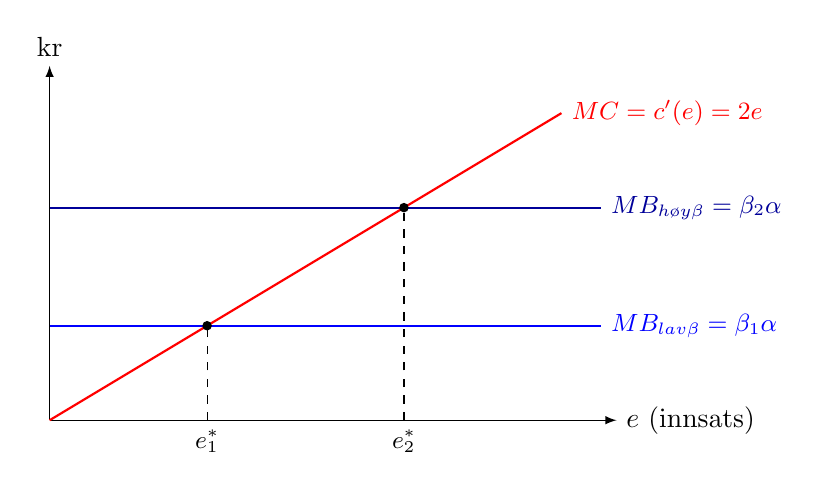
\begin{tikzpicture}[>=latex,scale=1.0]
  % Akser
  \draw[->] (0,0) -- (7.2,0) node[right] {$e$ (innsats)};
  \draw[->] (0,0) -- (0,4.5) node[above] {kr};
  % MB-linjer (konstant marginal benefit = beta*alpha)
  \draw[thick,blue] (0,1.2) -- (7,1.2) node[right] {\small $MB_{\text{lav }\beta}=\beta_1\alpha$};
  \draw[thick,blue!60!black] (0,2.7) -- (7,2.7) node[right] {\small $MB_{\text{høy }\beta}=\beta_2\alpha$};
  % MC = c'(e) = 2e (stigende)
  \draw[thick,red] (0,0) -- (6.5,3.9) node[right] {\small $MC=c'(e)=2e$};
  % Optimum 1
  \draw[dashed] (2.0,0) -- (2.0,1.2);
  \filldraw (2.0,1.2) circle (1.5pt);
  \node[below] at (2.0,0) {\small $e_1^{*}$};
  % Optimum 2
  \draw[dashed] (4.5,0) -- (4.5,2.7);
  \filldraw (4.5,2.7) circle (1.5pt);
  \node[below] at (4.5,0) {\small $e_2^{*}$};
\end{tikzpicture}
\caption{\textbf{Modell A -- agentens side.} Agenten velger $e^{*}$ der $MB=MC$, dvs.\ $\beta\alpha=c'(e)$. Når $\beta$ stiger fra $\beta_1$ til $\beta_2$, skifter $MB$ opp og optimal innsats $e^{*}$ flyttes til høyre. Fast lønn $W_0$ påvirker \emph{ikke} kurvene og dermed ikke $e^{*}$. [SLIDE -- BSZ kap.\ 15]}
\end{figure}

\subsection*{Modell B -- Prinsipalens side (optimal $\beta$)}

Prinsipalen maksimerer forventet profit $\mathbb{E}[\Pi]=\mathbb{E}[Q]-\mathbb{E}[W]$ underlagt to skranker:
\begin{itemize}\setlength{\itemsep}{1pt}
\item \emph{Incentive compatibility (IC):} agenten velger $e^{*}(\beta)$ som løser \eqref{eq:agent-foc}.
\item \emph{Participation (IR):} agentens $\mathrm{CE}\ge \overline{U}$ -- $W_0$ justeres slik at den ``binder''.
\end{itemize}
Når IR binder, ``betaler'' prinsipalen for både agentens innsatskostnad og risikopremien gjennom forventet lønn. Reduserer man problemet til valg av $\beta$, blir det:
\[
\max_{\beta}\;\;\underbrace{\alpha\,e^{*}(\beta)}_{\text{produksjonsgevinst}}\;-\;\underbrace{c\!\left(e^{*}(\beta)\right)}_{\text{innsatskostnad}}\;-\;\underbrace{\tfrac{r}{2}\beta^{2}\sigma^{2}}_{\text{risikopremie}}.
\]
Med $c(e)=e^{2}/(2k)$ slik at $c'(e)=e/k$ og dermed $e^{*}=k\beta\alpha$, blir FOC i $\beta$:
\begin{equation}\label{eq:beta-star}
\boxed{\;\beta^{*}\;=\;\dfrac{\alpha^{2}}{\alpha^{2}+r\sigma^{2}/k}\;=\;\dfrac{1}{1+r\sigma^{2}c''(e)/\alpha^{2}}\;}
\end{equation}
Dette er den klassiske Holmström-Milgrom-formelen (lineær kontrakt, CARA-nytte, normalfordelt støy). [BOK]

\textbf{Komparativ statikk.}
\begin{itemize}\setlength{\itemsep}{2pt}
\item $\beta^{*}\downarrow$ når agentens risikoaversjon $r$ stiger.
\item $\beta^{*}\downarrow$ når støyen $\sigma^{2}$ stiger -- jo mindre informativt $Q$ er om $e$, jo svakere insentiv.
\item $\beta^{*}\uparrow$ når produktiviteten $\alpha$ stiger.
\item $\beta^{*}\uparrow$ når marginalkostnaden av innsats $c''(e)$ faller (mindre konveks innsatskostnad).
\item Grensetilfeller: $r\to 0$ (risikonøytral agent) $\Rightarrow\beta^{*}\to 1$ (full residual claimancy, first-best); $\sigma^{2}\to 0$ (innsats kan ``leses ut'' av $Q$) $\Rightarrow\beta^{*}\to 1$.
\end{itemize}

\begin{figure}[h]
\centering
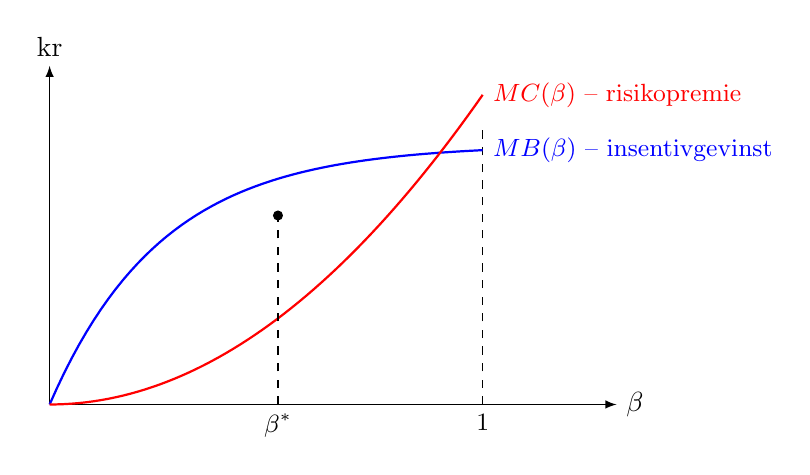
\begin{tikzpicture}[>=latex,scale=1.0]
  % Akser
  \draw[->] (0,0) -- (7.2,0) node[right] {$\beta$};
  \draw[->] (0,0) -- (0,4.3) node[above] {kr};
  \draw (5.5,0) node[below] {\small $1$};
  \draw[dashed] (5.5,0) -- (5.5,3.5);
  % Marginal benefit av β (konkav stigende): produksjonsgevinst minus innsatskostnad
  \draw[thick,blue,domain=0:5.5,samples=60]
    plot (\x,{3.3*(1-exp(-0.7*\x))}) node[right] {\small $MB(\beta)$ -- insentivgevinst};
  % Marginal cost av β (konveks stigende): risikopremie
  \draw[thick,red,domain=0:5.5,samples=60]
    plot (\x,{0.13*\x*\x}) node[right] {\small $MC(\beta)$ -- risikopremie};
  % Krysning (visuell): rundt β=2.8 i diagrammet
  \filldraw (2.9,2.4) circle (1.6pt);
  \draw[dashed] (2.9,0) -- (2.9,2.4);
  \node[below] at (2.9,0) {\small $\beta^{*}$};
\end{tikzpicture}
\caption{\textbf{Modell B -- prinsipalens side.} Prinsipalen velger $\beta^{*}$ der marginalt insentivutbytte ($MB(\beta)$, konkav stigende -- avtagende marginalgevinst av flere insentiver) lik marginal risikokostnad ($MC(\beta)$, konveks stigende -- risikopremien $\tfrac{r}{2}\beta^{2}\sigma^{2}$ stiger raskere enn lineært). $\beta^{*}<1$ i second-best; $\beta^{*}\to 1$ kun ved risikonøytral agent ($r=0$) eller perfekt observerbarhet ($\sigma^{2}=0$). [SLIDE -- BSZ kap.\ 15]}
\end{figure}

\subsection*{Slide-illustrasjon fra pensum}

\begin{figure}[h]
\centering

\includegraphics[width=0.55\linewidth]{BSZ_kap_15_2026/by_slide/slide_014/BSZ_kap_15_2026_slide_014_asset_01_image3.png}
\caption{Prinsipal-agent-modellen i BSZ kap.\ 15: $Q=\alpha e+\mu$, $W=W_0+\beta Q$, og effort-valget som funksjon av $\beta$. [SLIDE -- BSZ kap.\ 15, slide 14]}
\end{figure}

\subsection*{Kjerneforutsetninger}
\begin{itemize}\setlength{\itemsep}{1pt}
\item Lineær teknologi $Q=\alpha e+\mu$ med kjent $\alpha$ og normalfordelt $\mu$.
\item Lineær kontrakt $W=W_0+\beta Q$ (verifiserbar på $Q$).
\item CARA-nytte (eller $U=I-c(e)$) med konveks innsatskostnad $c(e)$, $c'(0)=0$, $c''(e)>0$.
\item Risikoavers agent ($r>0$), risikonøytral prinsipal (diversifisert).
\item Asymmetrisk informasjon: $e$ er ikke observerbart for prinsipalen (\thref{moral-hazard}{moral hazard}).
\item Reservasjonsnytte $\overline{U}$ utenfor virksomheten gitt (ytre arbeidsmarked).
\item Én oppgavedimensjon -- ingen multitasking (Holmström-Milgrom 1991).
\end{itemize}

\subsection*{Muligheter (hva modellen leverer)}
\begin{itemize}\setlength{\itemsep}{1pt}
\item En kvantitativ regel for hvor sterk insentivlønn skal være (\thref{incentive-coefficient}{$\beta^{*}$-formelen}).
\item En presis dekomponering av lønnen i en risikobærende og en innsatsdrivende del (\thref{fixed-vs-variable-pay}{$W_0$ vs.\ $\beta Q$}).
\item En formell forklaring på insentiv-risiko-trade-offen (\thref{risk-sharing}{risikodeling}).
\item Begrunnelsen for \thref{informativeness-principle}{informativeness-prinsippet}: redusér effektiv $\sigma^{2}$ ved bedre måltall.
\item Begrunnelsen for \thref{costly-contracting}{costly contracting}: second-best avviker fra \thref{costless-contracting}{costless contracting} nettopp pga.\ $r\sigma^{2}>0$.
\end{itemize}

\subsection*{Begrensninger og kritikk}
\begin{itemize}\setlength{\itemsep}{1pt}
\item Én-dimensjonal: i virkeligheten har agenten mange oppgaver med ulik målbarhet -- sterke insentiver på det målbare gir vridning bort fra det umålbare (Holmström-Milgrom 1991, ``equal compensation principle'').
\item Forutsetter at $Q$ er kontraktérbart -- mange resultater (kreativitet, samarbeid, kvalitet) er det ikke.
\item Risikoaversjonen $r$ og $\sigma^{2}$ må anslås -- vanskelig empirisk.
\item Ignorerer dynamikk: \emph{ratchet effect} (justert måltall år 2 dersom du leverer år 1), karriereinsentiver, reputasjon.
\item Atferdseffekter: \emph{crowding out} av indre motivasjon ved sterke ytre insentiver (Frey \& Jegen).
\item Antar én prinsipal -- multiple stakeholders (regulator, kreditorer, samfunn) bryter modellen.
\item Lineariteten er en bekvem antagelse; reelle bonusplaner har terskler, tak og opsjoner som skaper ikke-lineære insentiver og kan oppmuntre til gaming.
\item Forutsetter at agenten kjenner $\alpha$ og fordelingen av $\mu$ like godt som prinsipalen (mer realistisk: \thref{adverse-selection}{adverse selection} på begge sider).
\end{itemize}

\subsection*{Kobling til (a) risiko, (b) fast lønn, (c) $\beta$}
\begin{itemize}\setlength{\itemsep}{2pt}
\item \textbf{(a) Risiko:} Inngår i $\beta^{*}$ via $r\sigma^{2}$. Jo mer risikoavers agent og jo støyere måltall, jo lavere optimal $\beta$. Risikopremien $\tfrac{r}{2}\beta^{2}\sigma^{2}$ betales av prinsipalen gjennom forhøyet $W_0$. Se \thref{risk-sharing}{risk-sharing}.
\item \textbf{(b) Præstationsuafhængig løn $W_0$:} Faller ut av agentens FOC (vrir ikke innsats); dens rolle er å oppfylle IR-skranken og kompensere for risikopremien. Se \thref{fixed-vs-variable-pay}{fixed-vs-variable-pay}.
\item \textbf{(c) Incitamentskoefficient $\beta$:} Eneste parameter som vrir innsats. Trade-off mellom insentivgevinst og risikopremie gir formel \eqref{eq:beta-star}. Se \thref{incentive-coefficient}{incentive-coefficient}.
\end{itemize}

\subsection*{Eksempler}
\begin{itemize}\setlength{\itemsep}{2pt}
\item \textbf{Investment banking-trader:} $\sigma^{2}$ stor, men $\alpha$ også stor og trader-talenter er lite risikoaverse i porteføljen sin (har øvrig formue ofte diversifisert). Resultat: høy $\beta$, beskjeden $W_0$ -- bonuspuljen er hovedinntekten. [EKS]
\item \textbf{Offentlig sektor / lektor:} Output svært vanskelig å måle ($\sigma^{2}$ stort), agent er typisk risikoavers, og prinsipalen (stat) verdsetter likhet og normer. Resultat: $\beta\approx 0$, nesten alt $W_0$ (tarifflønn). [EKS]
\item \textbf{Selger på provisjon vs.\ butikksjef:} Selger har høyt og lett målbart $\alpha$ med relativt lite $\mu$ $\Rightarrow$ høy $\beta$. Butikksjef har bredere ansvarsområder hvor enkelte mål er mindre informative $\Rightarrow$ moderat $\beta$, betydelig $W_0$. [EKS]
\item \textbf{Equinor-CEO LTI:} Lederlønn med stor andel aksjebasert LTI, men også betydelig grunnlønn. $\sigma^{2}$ (oljepris) er stor og kompenseres delvis ved relative måltall (peer-gruppe) -- bruk av \thref{informativeness-principle}{informativeness-prinsippet}. [EKS]
\end{itemize}

\subsection*{Kobling til søyle og andre teorier}
Søyle: \STwo\ (måltallet $Q$) og \SThree\ (selve kontrakten $W_0+\beta Q$). Relaterte: \thref{principal-agent}{Principal-agent}, \thref{moral-hazard}{Moral hazard}, \thref{agency-costs}{Agency costs}, \thref{adverse-selection}{Adverse selection}, \thref{incentive-coefficient}{Incentive coefficient}, \thref{risk-sharing}{Risk sharing}, \thref{fixed-vs-variable-pay}{Fixed vs.\ variable pay}, \thref{costless-contracting}{Costless contracting}, \thref{costly-contracting}{Costly contracting}, \thref{informativeness-principle}{Informativeness-prinsippet}, \thref{specific-vs-general-knowledge}{Spesifik vs.\ generell viden} (driver fordi agenten kjenner $e$, prinsipalen ikke).

\paragraph{Brukt i spørsmål:} Q09.
